\documentclass[10pt,a4paper]{book}

\NewDocumentCommand\dawn{}{\texttt{dawn}}
\NewDocumentCommand\dusk{}{\texttt{dusk}}
\NewDocumentCommand\CPU{}{Intel Xeon\textregistered E5-2699 v3}

\book{D言語で実装する並列スケジューラ入門}{Parallel Work-Stealing Scheduler on D}{5}{D言語,並列処理,高性能計算,スレッド,HPC}

\begin{document}
\maketitle
\tableofcontents

\chapter{並列スケジューラの概念}

\textbf{並列処理}とは、長時間を要する計算の内容を分割して複数のプロセッサに分担させ、処理速度の改善を図る技術を指す。
並列処理には、\Algref{data}に示す\textbf{データ並列}による方法と、\Algref{task}に示す\textbf{タスク並列}による方法の2種類がある。

\begin{center}
\begin{minipage}{.49\textwidth}
\begin{algorithm}[H]
\caption{data parallelism.\label{alg:data}}
\begin{algorithmic}
\Procedure{$\mathrm{multiply}$}{matrices $A,B,C$}
\For{parallel $i$}
\For{parallel $j$}
\For{parallel $k$}
\State $c_{ij}\mathrel{{+}{=}}a_{ik}b_{kj}$
\EndFor
\EndFor
\EndFor
\EndProcedure
\end{algorithmic}
\end{algorithm}
\end{minipage}
\begin{minipage}{.49\textwidth}
\begin{algorithm}[H]
\caption{task parallelism.\label{alg:task}}
\begin{algorithmic}
\Procedure{$\mathrm{fibonacci}$}{integer $n$}
\If{$n>1$}
\State $t_1=\mathrm{fork}(\mathrm{fibonacci}(n-1))$
\State $t_2=\mathrm{fork}(\mathrm{fibonacci}(n-2))$
\Return $\mathrm{join}(t_1)+\mathrm{join}(t_2)$
\Else
\Return $n$
\EndIf
\EndProcedure
\end{algorithmic}
\end{algorithm}
\end{minipage}
\end{center}

前者はデータの分割に、後者はアルゴリズムの分割に着目するが、両者は背反な概念ではなく、単に着眼点の差である。
なお、プロセッサ内部では、命令の解読と実行と後処理など、\textbf{命令レベルの並列性}による逐次処理の高速化も行われる。

\section{データレベルの並列性}

処理の対象となるデータを分配して行う並列処理を、\textbf{データ並列処理}と呼ぶ。以下は、行列積を並列計算する例である。

\begin{Verbatim}{dlang}
void dmm_data(shared double[][] A, shared double[][] B, shared double[][] C) {
	import core.atomic, std.numeric, std.parallelism, std.range;
	foreach(i; parallel(iota(A.length))) {
	foreach(j; parallel(iota(B.length))) {
		C[i][j].atomicOp!"+="(A[i][].dotProduct(B[j][]));
	}
	}
}
\end{Verbatim}

単純な計算に限れば、CPUやGPUの\textit{single instruction multiple data}~(SIMD)~命令も、同様の並列処理を実現できる。
使用例を以下に示す。SIMD命令が処理するデータの量には限度があるため、\texttt{for}文の並列処理との併用が基本である。

\begin{Verbatim}{dlang}
void dmm_simd(shared double[][] A, shared double[][] B, shared double[][] C) {
	import core.simd, std.parallelism, std.range;
	foreach(i; parallel(iota(A.length)))
	foreach(j; parallel(iota(B.length))) {
		double2 u = 0;
		foreach(k; iota(0, A[i].length, 2)) {
			auto a = *cast(double2*) &A[i][k];
			auto b = *cast(double2*) &B[j][k];
			auto w = __simd(XMM.LODUPD, a);
			auto x = __simd(XMM.LODUPD, b);
			w = cast(double2)__simd(XMM.MULPD, w, x);
			u = cast(double2)__simd(XMM.ADDPD, w, u);
		}
		C[i][j] = u[0] + u[1];
	}
}
\end{Verbatim}

\section{タスクレベルの並列性}

関数など処理単位の非同期な実行による並列処理を、\textbf{タスク並列処理}と呼ぶ。非同期に実行される処理を\textbf{タスク}と呼ぶ。
非同期の実行を制御する仕組みが\textbf{スケジューラ}である。その主な役割は、動的な負荷分散である。\figref{fifo}に構成を示す。

\begin{figure}[h]
\centering
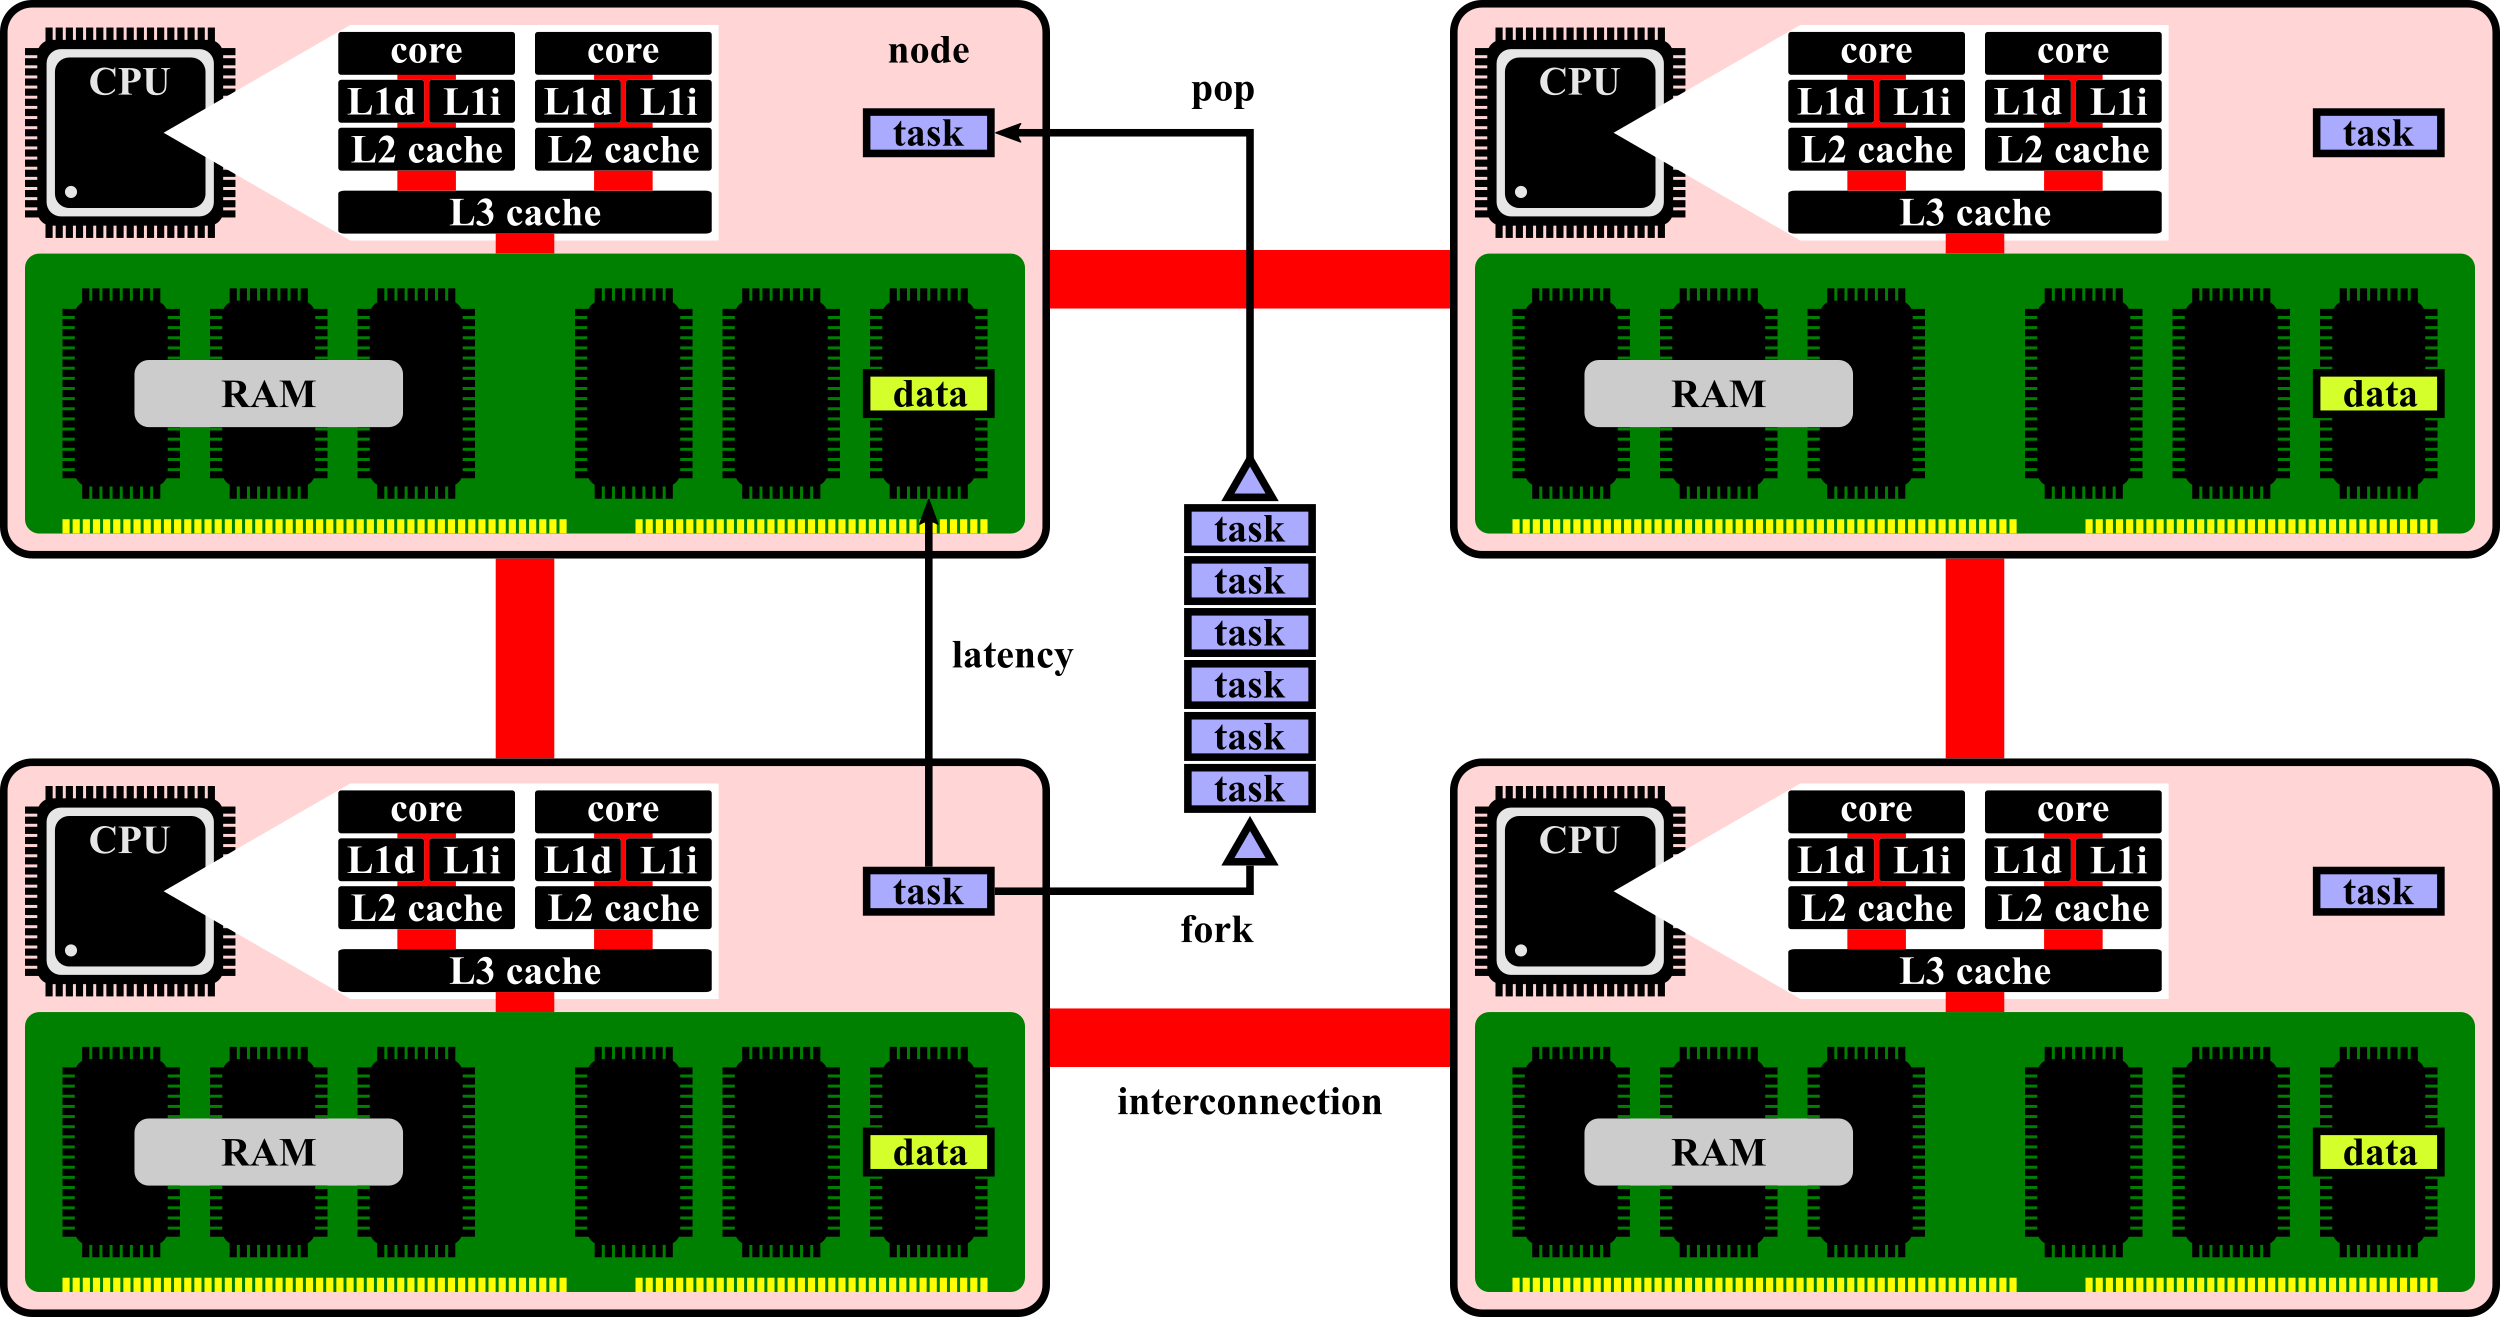
\includegraphics[width=\textwidth]{images/dawn.fifo.eps}
\caption{FIFO scheduler on shared-memory architecture.\label{fig:fifo}}
\end{figure}

現代の計算機は、プロセッサと主記憶が対をなす\textbf{ノード}の集合体であり、その間に、非対称な\textbf{メモリ空間}が共有される。
他のノードのデータを参照すると、\textbf{レイテンシ}で律速されるため、タスクが参照するデータは、局所化する必要がある。

\section{粗粒度なタスクの分配}

負荷分散だけに着目してタスクを分配すると、同じデータを参照するタスクが各ノードに分散し、参照の局所性を失う。
経験的には、再帰構造を持つタスクの末端を分配すると局所性が失われ、粗粒度な塊を分配すると局所性が保存される。

\section{ワークスティーリング\label{sect:filo}}

\figref{filo}に示す\textbf{ワークスティーリング}型のスケジューラでは、プロセッサは、自身が保有するタスクを後着順に実行する。

\begin{figure}[h]
\centering
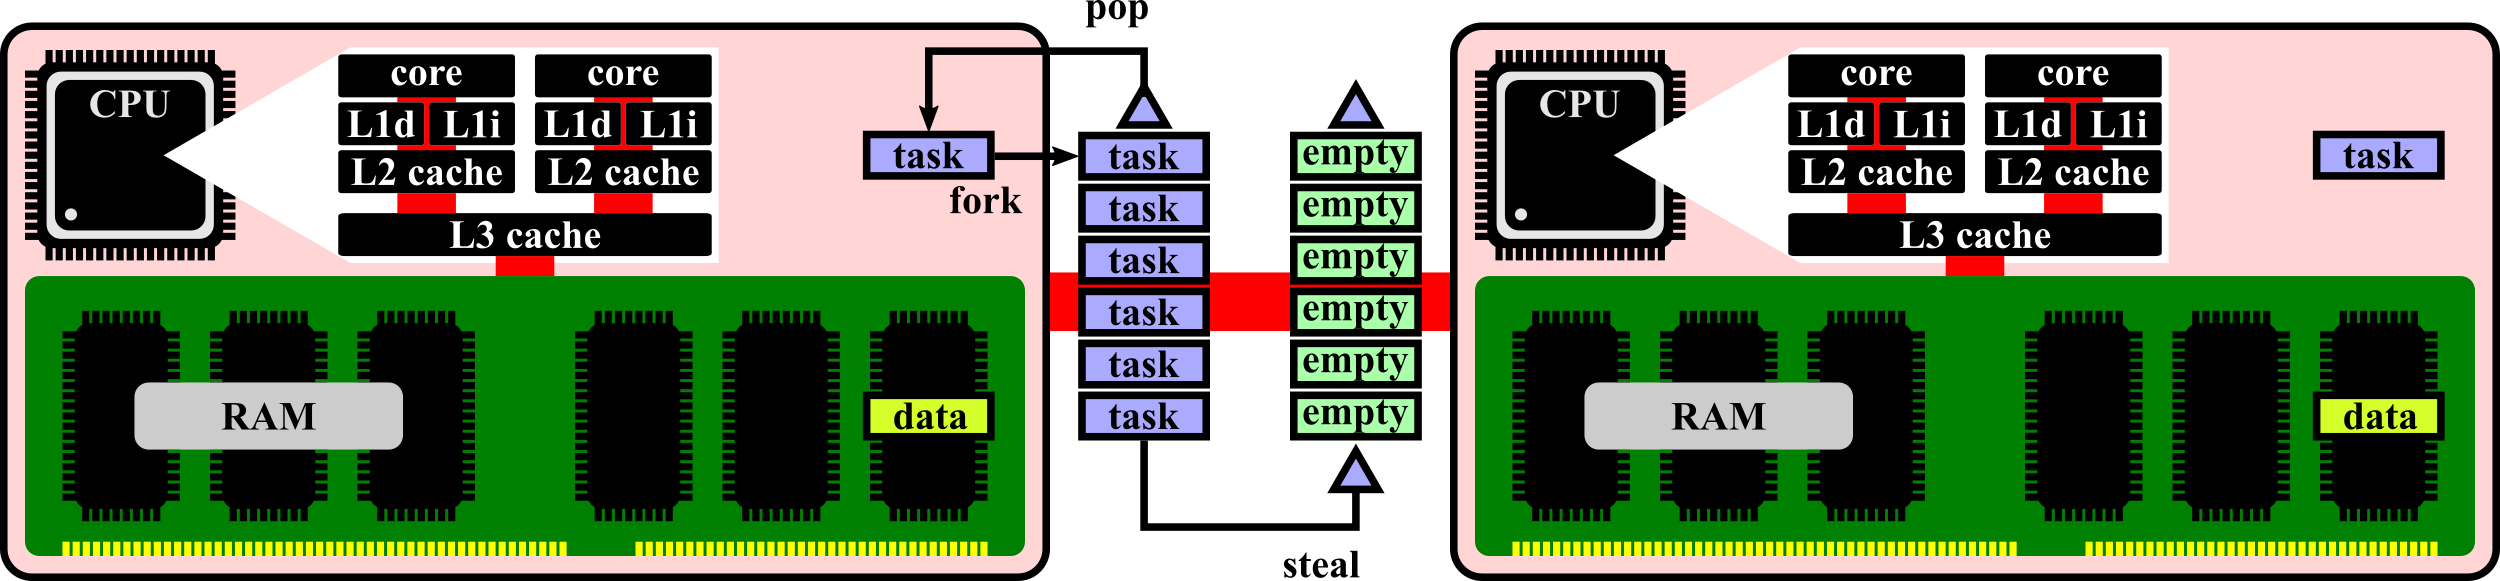
\includegraphics[width=\textwidth]{images/dawn.filo.eps}
\caption{work-stealing scheduler on shared-memory architecture.\label{fig:filo}}
\end{figure}

保有するタスクを消化した場合は、他のプロセッサにある、最も粗粒度な塊を、即ち、最古のタスクを奪って実行する。

\chapter{並列スケジューラの実装\label{chap:dawn}}

\sectref{filo}で議論した、ワークスティーリングを実装する。\chapref{dawn}に掲載する実装を順番に結合すると、完全な実装になる。
並列処理を開始する際に、プロセッサに識別番号を割り当てる。冒頭で、その識別番号の\textbf{スレッド局所変数}を宣言する。

\begin{Verbatim}{dlang}
private size_t coreId = -1;
\end{Verbatim}

\section{スケジューラ}

以下に実装する。\texttt{Ret}と\texttt{Args}は、並列実行するタスクが返す値と引数の型である。\texttt{boot}には、最初のタスクを与える。
\texttt{fork}は、タスクを分岐する。\texttt{join}は、指定のタスクが終わるまで\textbf{繁忙待機}し、必要なら他のプロセッサのタスクを奪う。

\begin{Verbatim}{dlang}
public shared class Dawn(Ret, Args...) {
	import std.parallelism, std.range;
	alias Ret function(Args) Func;
	private shared Deque[] stacks;
	private const size_t numCores;

	this(size_t numCores = totalCPUs) {
		this.numCores = numCores;
		foreach(i; iota(numCores)) {
			stacks ~= new shared Deque;
		}
	}

	public auto core(size_t index = coreId) {
		return stacks[index % numCores];
	}

	public auto fork(alias func)(Args args) {
		return core.add(new Task(&func, args));
	}

	public auto join(Task* task) {
		while(!task.isDone) spin(core.pop);
		return task.result;
	}

	private auto spin(Task* task) {
		if(task !is null) return task.invoke;
		foreach(index; iota(1, numCores)) {
			auto found = core(coreId + index).poll;
			if(found !is null) return found.invoke;
		}
	}

	public auto boot(alias func)(Args args) {
		auto root = new Task(&func, args);
		auto cpus = iota(numCores);
		foreach(c; taskPool.parallel(cpus, 1)) {
			if((coreId = c) == 0) root.invoke;
			else join(root);
		}
		return root.result;
	}
\end{Verbatim}

\section{タスクの実装}

タスクを表す関数と、その引数を格納する構造体を定義する。\texttt{invoke}は、指定された関数を実行し、返り値を保存する。
命令の\textbf{アウトオブオーダー実行}が原因で、関数を実行する前に\texttt{done}が書き換わる場合があり、\textbf{メモリバリア}で対策した。

\begin{Verbatim}{dlang}
	private static final struct Task {
		import core.atomic;
		private bool done;
		private Func func;
		private Args args;
		private Ret value;

		this(Func func, Args args) {
			this.func = func;
			this.args = args;
			this.done = false;
		}

		public bool isDone() {
			return atomicLoad(*(cast(shared) &done));
		}

		public void invoke() {
			value = func(args);
			atomicStore(*(cast(shared) &done), true);
		}

		public auto result() {
			return value;
		}
	}
\end{Verbatim}

\section{キューの実装}

各プロセッサが保有するタスクを格納する両端キューを実装する。プロセッサ間での競合を防ぐため、\textbf{排他制御}を行う。

\begin{Verbatim}{dlang}
	private synchronized final class Deque {
		private Task*[] buffer;

		public Task* add(Task* task) {
			buffer ~= cast(shared) task;
			return task;
		}

		public Task* pop() {
			if(!buffer.empty) {
				auto task = buffer[$-1];
				buffer = buffer[0..$-1];
				return cast(Task*) task;
			} else return null;
		}

		public Task* poll() {
			if(!buffer.empty) {
				auto task = buffer[0];
				buffer = buffer[1..$];
				return cast(Task*) task;
			} else return null;
		}
	}
}
\end{Verbatim}

\chapter{キャッシュ効率の最適化\label{chap:cache}}

並列処理では、台数効果も重要だが、逐次処理の性能も重要である。特に、参照局所性を意識した最適化が、必須となる。

\section{キャッシュミス率の抑制}

\textbf{キャッシュ}は、低容量で高速な記憶装置である。主記憶の値を読むと、周囲の連続した領域がキャッシュに複製される。
その恩恵で、配列の要素を順番に処理すると、複製が利用できる確率が高まり、処理を高速化できる。行列積で実験する。

\begin{Verbatim}{dlang}
import std.datetime.stopwatch, std.range, std.random, std.stdio;

const size_t N = 256;
double[N][N] A, B, C;

void dmm_slow() {
	foreach(i; iota(N)) foreach(j; iota(N)) foreach(k; iota(N)) C[i][j] += A[i][k] * B[k][j];
}

void dmm_fast() {
	foreach(i; iota(N)) foreach(j; iota(N)) foreach(k; iota(N)) C[i][j] += A[i][k] * B[j][k];
}

void main() {
	const size_t trial = 10;
	foreach(i; iota(N)) foreach(j; iota(N)) A[i][j] = uniform(0, 1);
	foreach(i; iota(N)) foreach(j; iota(N)) B[i][j] = uniform(0, 1);
	foreach(i; iota(N)) foreach(j; iota(N)) C[i][j] = uniform(0, 1);
	auto slow = 2.0 * trial / benchmark!dmm_slow(trial)[0].total!"nsecs" * N * N * N;
	auto fast = 2.0 * trial / benchmark!dmm_fast(trial)[0].total!"nsecs" * N * N * N;
	writefln("slow: %.5fGFLOPS", slow);
	writefln("fast: %.5fGFLOPS", fast);
}
\end{Verbatim}

\CPU{}の結果を示す。動作周波数を考えれば、連続的な参照の場合に、ほぼ理論的な最高性能に達した。
ただし、並列処理で、複数のプロセッサが同時に主記憶を参照し、\textbf{バス}が混雑する場合は、理論性能の発揮が困難になる。

\begin{Verbatim}{bash}
$ ldc -O -release -boundscheck=off -of=dmm dmm.d
$ taskset -c 0 ./dmm
slow: 0.84760GFLOPS
fast: 2.01925GFLOPS
\end{Verbatim}

複数のプロセッサが変数を共有し、内蔵のキャッシュに保持すると、その値をプロセッサ間で同期させる必要が生じる。
この同期は、キャッシュの値を無効化し、主記憶を読み直す動作で実現するので、頻繁に生じれば、律速の要因となる。

\section{キャッシュの競合の抑制}

複数のプロセッサが共有変数に値を書き込み、交互にキャッシュが無効化される状態を、\textbf{フォルスシェアリング}と呼ぶ。
その対策を以下に示す。行列の各行の空の領域を設定し、記憶領域を分離することで、意図せず共有される事態を防ぐ。

\begin{Verbatim}{dlang}
immutable size_t N = 8192;
immutable size_t PAD = 32;
shared double[N][N + PAD] A, B, C;
\end{Verbatim}

\chapter{行列積の並列処理の評価\label{chap:dmm}}

\chapref{dmm}では、行列積の処理速度の計測を通じて、\chapref{dawn}で実装したスケジューラを利用した場合の\textbf{台数効果}を確認する。
具体的には、正方行列$A,B$の積だが、行列$B$のキャッシュミスを抑制するため、行列$B$を転置した$A\trans{B}$の形式とする。

\begin{Verbatim}{dlang}
import core.atomic, std.algorithm, std.numeric, std.parallelism, std.random, std.range, std.stdio;
\end{Verbatim}

まず、行列の配列を宣言する。各行の末尾に空の領域を設定し、\chapref{cache}で学んだフォルスシェアリングによる律速を防ぐ。
また、\chapref{dawn}で実装したスケジューラの変数も宣言する。実行時にプロセッサ数が決まるので、初期化は実行時に行う。

\begin{Verbatim}{dlang}
const int N = 8192;
const int PAD = 32;
const int PADDED = N + PAD;
shared double[N * PADDED] A;
shared double[N * PADDED] B;
shared double[N * PADDED] C = 0;
shared Dawn!(int, int, int, int, int, int, int, int) sched;
\end{Verbatim}

次に、部分行列の積の逐次処理を実装する。1行1列に至るまで並列化すると効率が悪化するので、逐次処理を併用する。

\begin{Verbatim}{dlang}
void dmm_leaf(int i1, int i2, int j1, int j2, int k1, int k2) {
	foreach(i,iN; enumerate(iota(i1 * PADDED, i2 * PADDED, PADDED), i1))
	foreach(j,jN; enumerate(iota(j1 * PADDED, j2 * PADDED, PADDED), j1))
		C[iN+j].atomicOp!"+="(A[iN+k1..iN+k2].dotProduct(B[jN+k1..jN+k2]));
}
\end{Verbatim}

\section{提案実装による並列化\label{sect:dmm:dawn}}

行列を再帰的に分割し、部分行列を計算するタスクを分岐して、分割統治法とワークスティーリングで並列処理を行う。
最長軸を分割し、部分行列が正方行列に近付くほど、同じ計算量でも参照が局所化され、キャッシュミスを抑制できる。

\begin{Verbatim}{dlang}
int dmm_dawn(int i1, int i2, int j1, int j2, int k1, int k2, int grain) {
	auto axes = [i2 - i1, j2 - j1, k2 - k1];
	if(axes.maxElement <= grain) {
		dmm_leaf(i1, i2, j1, j2, k1, k2);
	} else if(axes.maxIndex == 0) {
		auto t1 = sched.fork!dmm_dawn(i1, (i1+i2)/2, j1, j2, k1, k2, grain);
		auto t2 = sched.fork!dmm_dawn((i1+i2)/2, i2, j1, j2, k1, k2, grain);
		sched.join(t1);
		sched.join(t2);
	} else if(axes.maxIndex == 1) {
		auto t1 = sched.fork!dmm_dawn(i1, i2, j1, (j1+j2)/2, k1, k2, grain);
		auto t2 = sched.fork!dmm_dawn(i1, i2, (j1+j2)/2, j2, k1, k2, grain);
		sched.join(t1);
		sched.join(t2);
	} else if(axes.maxIndex == 2) {
		auto t1 = sched.fork!dmm_dawn(i1, i2, j1, j2, k1, (k1+k2)/2, grain);
		auto t2 = sched.fork!dmm_dawn(i1, i2, j1, j2, (k1+k2)/2, k2, grain);
		sched.join(t1);
		sched.join(t2);
	}
	return 0;
}
\end{Verbatim}

\section{既存実装による並列化}

提案実装と比較するため、D言語の標準ライブラリに含まれる\texttt{TaskPool}を利用して、同じ手順で行列積を並列化する。
提案実装との比較により、\figref{fifo}の集中管理型の並列処理と、\figref{filo}の分散管理型の並列処理の、性能差を検証する。

\begin{Verbatim}{dlang}
void dmm_pool(int i1, int i2, int j1, int j2, int k1, int k2, int grain) {
	auto axes = [i2 - i1, j2 - j1, k2 - k1];
	if(axes[axes.maxIndex] <= grain) {
		dmm_leaf(i1, i2, j1, j2, k1, k2);
	} else if(axes.maxIndex == 0) {
		auto t1 = task!dmm_pool(i1, (i1+i2)/2, j1, j2, k1, k2, grain);
		auto t2 = task!dmm_pool((i1+i2)/2, i2, j1, j2, k1, k2, grain);
		taskPool.put(t1);
		taskPool.put(t2);
		t1.workForce;
		t2.workForce;
	} else if(axes.maxIndex == 1) {
		auto t1 = task!dmm_pool(i1, i2, j1, (j1+j2)/2, k1, k2, grain);
		auto t2 = task!dmm_pool(i1, i2, (j1+j2)/2, j2, k1, k2, grain);
		taskPool.put(t1);
		taskPool.put(t2);
		t1.workForce;
		t2.workForce;
	} else if(axes.maxIndex == 2) {
		auto t1 = task!dmm_pool(i1, i2, j1, j2, k1, (k1+k2)/2, grain);
		auto t2 = task!dmm_pool(i1, i2, j1, j2, (k1+k2)/2, k2, grain);
		taskPool.put(t1);
		taskPool.put(t2);
		t1.workForce;
		t2.workForce;
	}
}
\end{Verbatim}

\section{反復処理による並列化\label{sect:dmm:grid}}

再帰的な分割統治を実施せず、行列を3軸で末端粒度まで分割し、逐次的に暇なプロセッサに分配する方法を実装する。

\begin{Verbatim}{dlang}
void dmm_gr3d(int i1, int i2, int j1, int j2, int k1, int k2, int grain) {
	const int iN = (i2 - i1) / grain;
	const int jN = (j2 - j1) / grain;
	const int kN = (k2 - k1) / grain;
	foreach(ch; parallel(iota(0, iN * jN * kN), 1)) {
		const int i = i1 + ch / kN / jN * grain;
		const int j = j1 + ch / kN % jN * grain;
		const int k = k1 + ch % kN * grain;
		dmm_leaf(i, i + grain, j, j + grain, k, k + grain);
	}
}
\end{Verbatim}

行列を2軸で分割した場合も実装する。$k$軸で分割せず、$i,j$軸を並列化した場合である。部分行列は$k$軸のみ長くなる。

\begin{Verbatim}{dlang}
void dmm_gr2d(int i1, int i2, int j1, int j2, int k1, int k2, int grain) {
	const int iN = (i2 - i1) / grain;
	const int jN = (j2 - j1) / grain;
	foreach(ch; parallel(iota(0, iN * jN), 1)) {
		const int i = i1 + ch / jN * grain;
		const int j = j1 + ch % jN * grain;
		dmm_leaf(i, i + grain, j, j + grain, k1, k2);
	}
}
\end{Verbatim}

\section{台数効果の評価と解釈}

最後に、\texttt{main}関数を実装する。行列積に含まれる乗算と加算の回数を処理時間で割ると、処理速度のflops値が求まる。

\begin{Verbatim}{dlang}
void main() {
	import std.datetime.stopwatch;
	defaultPoolThreads = totalCPUs;
	sched = new typeof(sched);
	foreach(i; iota(A.length)) A[i] = uniform(0, 1);
	foreach(i; iota(B.length)) B[i] = uniform(0, 1);
	auto watch = StopWatch(AutoStart.yes);
	sched.boot!dmm_dawn(0, N, 0, N, 0, N, 128);
	writeln(2.0 / watch.peek.total!"nsecs" * N * N * N, "GFLOPS");
}
\end{Verbatim}

以上で、行列積の並列処理が完成した。以下の操作でコンパイルする。最適化は有効に、実行時の境界検査は無効にする。

\begin{Verbatim}{bash}
$ ldc -O -release -boundscheck=off -of=dmm dmm.d
$ for c in {0..35}; do taskset -c 0-$c ./dmm; done
\end{Verbatim}

\figref{dawn.dmm}は、2個の\CPU{}を搭載した、NUMA型の共有メモリ環境で、台数効果を描画した結果である。
2軸での分割は、並列化の費用対効果を大幅に損ねた。再帰的な並列化とワークスティーリングの併用は、効果的である。

\begin{figure}[h]
\centering
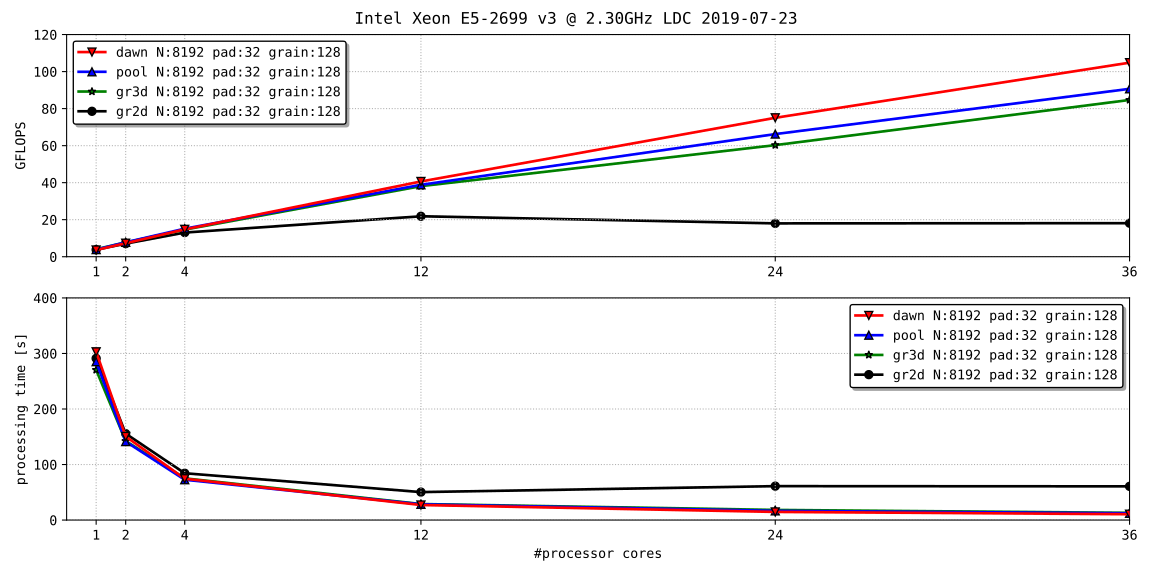
\includegraphics[width=\textwidth]{scales/dawn.dmm.rank8192.gran128.pad32.ldc.xeon.e5.2699.v3.core36.eps}
\caption{dense matrix multiplication, $8192\times8192\times8192$.\label{fig:dawn.dmm}}
\end{figure}

同じ並列化でも、提案実装と既存実装の性能には差がある。その差を解釈する。まず、排他制御の所要時間を$D$とする。
排他制御を$M/D/1$の待ち行列とし、$N$個のプロセッサが\textbf{ポアソン到着}すると、待ち時間$w$の期待値は\eqref{md1n.w}となる。
%
\begin{alignat}{1}
\label{eq:md1n.w}
w &= \seq{N-1-\frac{1}{\rho b_{N-1}}\tup{\sum_{n=0}^{N-1}b_n-N}}D,\\
b_n &= \sum_{k=0}^n\frac{(-1)^k}{k!}(n-k)^ke^{(n-k)\rho}\rho^k,\\
\rho &= \lambda D.
\end{alignat}
%
特に細粒度の並列処理の場合は、既存実装のままプロセッサを増強すると、到着率$\lambda$が増加して、待ち時間が急増する。
逆に、常に疎粒度のタスクを奪う提案実装では、到着率$\lambda$が抑制される。\eqref{md1n.w}は、Brun~\&~Garcia~(2000)に従った。

\chapter{高性能並列処理系の紹介\label{chap:dusk}}

\chapref{dusk}で解説する\dusk{}は、\textit{non~uniform~memory~access}~(NUMA)~型の共有メモリ環境を指向したスケジューラである。

\section{利用方法\label{sect:dusk.api}}

\dusk{}の実装は、GitHubで無償公開している。以下の操作でインストールできる。依存性の都合から、UNIX環境に限る。

\begin{Verbatim}{bash}
$ git clone https://github.com/autodyne/dusk
# make build install -C dusk
# ldconfig
\end{Verbatim}

\dusk{}は、\texttt{gcc}と\texttt{clang}と\texttt{icc}の全てのコンパイラで動作を確認した。\texttt{libdusk.so}が本体で、以下の操作で利用できる。

\begin{Verbatim}{bash}
$ g++ -ldusk -std=c++11 your_program.cpp
\end{Verbatim}

\dusk{}のAPIは、\texttt{dusk.hpp}を通じて、以下に解説する\texttt{launch}と\texttt{salvo}と\texttt{burst}の3個のテンプレート関数を提供する。
\texttt{launch}は、指定された関数を起点に並列処理を開始し、待機する。\texttt{salvo}は、\texttt{f(a)}と\texttt{f(b)}を並列に実行し、待機する。

\begin{Verbatim}{C++}
void sun::launch(void(*pad)(void));
template<typename Arg> void sun::salvo(void (*f)(Arg), Arg a, Arg b);
template<typename Idx> void sun::burst(Idx range, void (*body)(Idx));
\end{Verbatim}

\texttt{burst}は、データ並列処理の実装で、指定された個数だけ関数を並列実行し、待機する。関数には、通し番号が渡される。
以上の関数の実体を、以下に示す。仕組みは\chapref{dawn}と同等だが、\textbf{ロックフリー}な排他制御も実装して、高性能化を図った。

\begin{Verbatim}{C++}
namespace sun {
class Task;

void launch(void (*pad)(void)) {
	using funct = param(*)(param);
	root((funct)pad, (void*)NULL);
}

template<typename Arg> void salvo(void (*f)(Arg), Arg a, Arg b) {
	using funct = void*(*)(void*);
	extern Task* dawn(funct fn, void* a);
	extern void* dusk(Task* waitingtask);
	auto t1 = dawn((funct) f, (void*) a); // fork
	auto t2 = dawn((funct) f, (void*) b); // fork
	dusk(t2); // join
	dusk(t1); // join
}

template<typename Idx> void burst(Idx round, void (*body)(Idx)) {
	using funct = void*(*)(void*);
	extern Task* dawn(funct fn, void* a);
	extern void* dusk(Task* waitingtask);
	Task** th = new Task*[round];
	for(Idx i=0;i<round;i++) th[i] = dawn((funct)body, (void*)i);
	for(Idx i=0;i<round;i++) dusk(th[i]);
	delete th;
}
};
\end{Verbatim}

\section{環境変数}

以下の環境変数により、論理プロセッサ数や負荷分散の戦術や、各プロセッサに格納可能なタスクの個数を変更できる。

\begin{Verbatim}{bash}
$ export DUSK_WORKER_NUM=80
$ export DUSK_TACTICS=PDRWS
$ export DUSK_STACK_SIZE=64
\end{Verbatim}

環境変数\texttt{DUSK\_TACTICS}に設定可能な戦術と、その効果を\tabref{tactics}に示す。特に指定しなければ、\texttt{PDRWS}が選択される。
細粒度の並列処理では、\texttt{QUEUE}よりも\texttt{PDRWS}が優位である。\texttt{ADRWS}の\texttt{PDRWS}に対する優位性は、現時点では曖昧である。

\begin{table}[h]
\centering
\caption{\texttt{DUSK\_TACTICS}\label{tab:tactics}}
\begin{tabular}{>{\ttfamily}c>{\ttfamily}cl} \toprule
設定値 & 負荷分散 & 初期タスクの分配 \\ \midrule[.8pt]
QUEUE & FIFO(1) & キューから全プロセッサに分配 \\ \midrule
PDRWS & FILO(N) & 繁忙状態のプロセッサから奪取 \\ \midrule
ADRWS & FILO(N) & 幅優先的に全プロセッサに分配 \\ \bottomrule
\end{tabular}
\end{table}

\section{性能測定}

2個の\CPU{}を搭載したNUMA型の共有メモリ環境で、行列積の速度を測定し、台数効果を評価した。

\begin{Verbatim}{bash}
$ make -C dusk/test/dmm
$ ./dusk/test/dmm/dmm.plot
\end{Verbatim}

\figref{dusk.dmm}に結果を示す。MeltdownやSpectreの対策により、\CPU{}の性能が制限される前に測定した。

\begin{figure}[h]
\centering
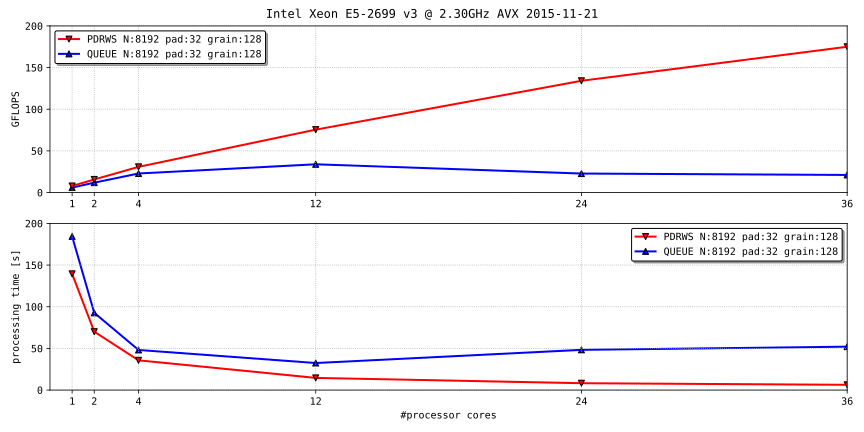
\includegraphics[width=\textwidth]{scales/dusk.dmm.rank8192.gran128.pad32.avx.xeon.e5.2699.v3.core36.eps}
\caption{dense matrix multiplication, $8192\times8192\times8192$, vectorized by AVX.\label{fig:dusk.dmm}}
\end{figure}

\texttt{PDRWS}は、\sectref{dmm:dawn}のタスク並列処理に相当し、3軸を粒度$128$まで再帰的に並列化して、末端でSIMD命令を使用した。
\texttt{QUEUE}は、\sectref{dmm:grid}のデータ並列処理に相当し、2軸を粒度$128$まで格子状に並列化して、同様にSIMD命令を使用した。

\end{document}
